%% For double-blind review submission, w/o CCS and ACM Reference (max submission space)
\documentclass[sigplan,10pt,review,anonymous]{acmart}
\settopmatter{printfolios=true,printccs=false,printacmref=false}
%% For double-blind review submission, w/ CCS and ACM Reference
%\documentclass[sigplan,review,anonymous]{acmart}\settopmatter{printfolios=true}
%% For single-blind review submission, w/o CCS and ACM Reference (max submission space)
%\documentclass[sigplan,review]{acmart}\settopmatter{printfolios=true,printccs=false,printacmref=false}
%% For single-blind review submission, w/ CCS and ACM Reference
%\documentclass[sigplan,review]{acmart}\settopmatter{printfolios=true}
%% For final camera-ready submission, w/ required CCS and ACM Reference
%\documentclass[sigplan]{acmart}\settopmatter{}


%% Conference information
%% Supplied to authors by publisher for camera-ready submission;
%% use defaults for review submission.
%\acmConference[ARRAY'22]{ACM SIGPLAN Conference on Programming Languages}{June 13, 2022}{San Diego, CA, USA}
%\acmYear{2018}
%\acmISBN{} % \acmISBN{978-x-xxxx-xxxx-x/YY/MM}
%\acmDOI{} % \acmDOI{10.1145/nnnnnnn.nnnnnnn}
%\startPage{1}

%% Copyright information
%% Supplied to authors (based on authors' rights management selection;
%% see authors.acm.org) by publisher for camera-ready submission;
%% use 'none' for review submission.
\setcopyright{none}
%\setcopyright{acmcopyright}
%\setcopyright{acmlicensed}
%\setcopyright{rightsretained}
%\copyrightyear{2018}           %% If different from \acmYear

\usepackage{dsfont}
\usepackage{stmaryrd}

%% Bibliography style
\bibliographystyle{acmart}

\usepackage{dsfont}
\usepackage{stmaryrd}
\usepackage{colortbl}
\usepackage{hyperref}

\usepackage{amsmath}
\DeclareMathOperator*{\argmax}{argmax}
\DeclareMathOperator*{\argmin}{argmin}
\usepackage{amssymb}

\usepackage[dvipsnames, table]{xcolor}
\usepackage{textcomp}

% Packages
\usepackage[pdf]{graphviz}
\usepackage{mathrsfs}

\newcommand*\circled[1]{\tikz[baseline=-0.1cm]{
  \node[shape=circle,draw,inner sep=0.48pt] (char) {\fontsize{7}{12}\textsf{#1}};}}

\DeclareMathAlphabet{\mathcal}{OMS}{cmsy}{m}{n}
\usepackage{cancel}
\newcommand\ccancel[2][red]{\renewcommand\CancelColor{\color{#1}}\cancel{#2}}
\newcommand{\nDownarrow}{\ensuremath{\text{ }\cancel{\Downarrow}\text{ }}}
\usepackage{centernot}

\usepackage{pgfplots, pgfplotstable}
\pgfplotsset{compat=1.7}
\usepgfplotslibrary{fillbetween}
\usetikzlibrary{patterns}
\pgfmathdeclarefunction{gauss}{2}{\pgfmathparse{1/(#2*sqrt(2*pi))*exp(-((x-#1)^2)/(2*#2^2))}}
\pgfmathdeclarefunction{nil}{1}{\pgfmathparse{0.001}}

\usepackage{arydshln}
\usepackage{adjustbox}
\usepackage{enumerate}
\usepackage{enumitem}
\usepackage{tikz-cd}
\usetikzlibrary{calc}
\usepackage{amsfonts}
%\usepackage{prooftrees}
\usepackage{bussproofs}
\renewcommand{\sectionautorefname}{\S}
\renewcommand{\subsectionautorefname}{\S}
\usepackage{float}

\usepackage{tikz-3dplot}
\usetikzlibrary{3d}
\usetikzlibrary{calligraphy}
\newif\ifshowcellnumber
\showcellnumbertrue

\usepackage{algorithm}
\usepackage{algpseudocode}
\usepackage{algorithmicx}
\usepackage{sourcecodepro}
\usepackage{tikz-qtree}
\usepackage{amsthm}
\usepackage{bm}
\usetikzlibrary{bayesnet}
\usetikzlibrary{arrows}
\usepackage{subcaption}
\usetikzlibrary{backgrounds}
\usetikzlibrary{tikzmark}
\usetikzlibrary{hobby}

\usepackage{mwe}

\newcommand{\E}{\mathbb{E}}
\newcommand{\Var}{\mathrm{Var}}
\newcommand{\Cov}{\mathrm{Cov}}

\newcommand{\CompOrder}{\mathcal{O}}
\def\graphspace{\mathbf{G}}
\def\Uniform{\mbox{\rm Uniform}}
\def\Gaussian{\mbox{\rm Gaussian}}
\def\Bernoulli{\mbox{\rm Bernoulli}}
\def\Dirichlet{\mbox{\rm Dirichlet}}

\usepackage{mathtools}% superior to amsmath
\usepackage{tikz}
% Packages
\usepackage{listings}
\DeclareRobustCommand{\hlred}[1]{{\sethlcolor{pink}\hl{#1}}}
\usepackage{fontspec}

\setmonofont[Scale=0.8]{JetBrainsMono}[
  Contextuals={Alternate},
  Path=./font/,
  Extension = .ttf,
  UprightFont=*-Regular,
  BoldFont=*-Bold,
  ItalicFont=*-Italic,
  BoldItalicFont=*-BoldItalic
]

\usepackage[skins,breakable,listings]{tcolorbox}

\lstdefinelanguage{kotlin}{
  comment=[l]{//},
  commentstyle={\color{gray}\ttfamily},
  emph={delegate, filter, firstOrNull, forEach, it, lazy, mapNotNull, println, repeat, assert, with, head, tail, len, return@},
  numberstyle=\noncopyable,
  identifierstyle=\color{black},
  keywords={abstract, actual, as, as?, break, by, class, companion, continue, data, do, dynamic, else, enum, expect, false, final, for, fun, get, if, import, in, infix, interface, internal, is, null, object, open, operator, override, package, private, public, return, sealed, set, super, suspend, this, throw, true, try, catch, typealias, val, var, vararg, when, where, while, tailrec, reified},
  keywordstyle={\bfseries},
  morecomment=[s]{/*}{*/},
  morestring=[b]",
  morestring=[s]{"""*}{*"""},
  ndkeywords={@Deprecated, @JvmField, @JvmName, @JvmOverloads, @JvmStatic, @JvmSynthetic, Array, Byte, Double, Float, Boolean, Int, Integer, Iterable, Long, Runnable, Short, String, int},
  ndkeywordstyle={\bfseries},
  sensitive=true,
  stringstyle={\ttfamily},
  literate={`}{{\char0}}1,
  escapeinside={(*@}{@*)}
}
\lstdefinelanguage{tidy}{
  comment=[l]{//},
  commentstyle={\color{gray}\ttfamily},
  emph={|, ->, ---},
  emphstyle={\color{red}},
  identifierstyle=\color{black},
  keywords={\|, ->, ---},
  otherkeywords={|,->},
  morekeywords={|,->},
  keywordstyle={\color{blue}\bfseries},
  morecomment=[s]{/*}{*/},
  morestring=[b]",
  morestring=[s]{"""*}{*"""},
  ndkeywords={@Deprecated, @JvmField, @JvmName, @JvmOverloads, @JvmStatic, @JvmSynthetic, Array, Byte, Double, Float, Int, Integer, Iterable, Long, Runnable, Short, String},
  ndkeywordstyle={\color{orange}\bfseries},
  sensitive=true,
  stringstyle={\color{green}\ttfamily},
  literate={`}{{\char0}}1
}

%%%%%%%%%%%%%%%%%%%%%%%%%%%%%%%%%%%%%%%%%%%
%
% Color boxes
%
%%%%%%%%%%%%%%%%%%%%%%%%%%%%%%%%%%%%%%%%%%%

\tcbset{
  enhanced jigsaw,
  breakable,
  listing only,
%  boxsep=-1pt,
%  top=-1pt,
  bottom=0.1cm,
  right=0.5cm,
  overlay first={
    \node[black!50] (S) at (frame.south) {\Large\ding{34}};
    \draw[dashed,black!50] (frame.south west) -- (S) -- (frame.south east);
  },
  overlay middle={
    \node[black!50] (S) at (frame.south) {\Large\ding{34}};
    \draw[dashed,black!50] (frame.south west) -- (S) -- (frame.south east);
    \node[black!50] (S) at (frame.north) {\Large\ding{34}};
    \draw[dashed,black!50] (frame.north west) -- (S) -- (frame.north east);
  },
  overlay last={
    \node[black!50] (S) at (frame.north) {\Large\ding{34}};
    \draw[dashed,black!50] (frame.north west) -- (S) -- (frame.north east);
  },
  before={\par\vspace{5pt}},
  after={\par\vspace{\parskip}\noindent}
}

\definecolor{slightgray}{rgb}{0.90, 0.90, 0.90}

\usepackage{soul}
\makeatletter
\def\SOUL@hlpreamble{%
  \setul{}{3.0ex}%
  \let\SOUL@stcolor\SOUL@hlcolor%
  \SOUL@stpreamble%
}
\makeatother

\newcommand{\inline}[1]{%
  \begingroup%
  \sethlcolor{slightgray}%
  \hl{\ttfamily\footnotesize #1}%
  \endgroup
}

\newcommand{\tinline}[1]{%
  \begingroup%
  \sethlcolor{slightgray}%
  \hl{\ttfamily\tiny #1}%
  \endgroup
}

\newtcblisting{halftidyinput}[1][]{%
  left skip=0.7cm,
  left=0.35cm,
  width=6cm,
%  left=-0.01cm,
  top=-0.1cm,
  bottom=-0.35cm,
  listing options={
    language=tidy,
    basicstyle=\ttfamily\small,
%numberstyle=\footnotesize,
    showstringspaces=false,
    tabsize=2,
    breaklines=true,
    numbers=none,
    inputencoding=utf8,
    escapeinside={(*@}{@*)},
    #1
  },
  underlay unbroken and first={%
    \path[draw=none] (interior.north west) rectangle node[white]{
\includegraphics[width=4mm]{../figures/tidyparse_logo.png}} ([xshift=-10mm,yshift=-7mm]interior.north west);
  }
}

\newtcblisting{wholetidyinput}[1][]{%
  left skip=0.7cm,
  left=0.35cm,
  top=0.1cm,
  middle=0mm,
  boxsep=0mm,
  listing options={
    language=tidy,
    basicstyle=\ttfamily\small,
%numberstyle=\footnotesize,
    showstringspaces=false,
    tabsize=2,
    breaklines=true,
    numbers=none,
    inputencoding=utf8,
    escapeinside={(*@}{@*)},
    #1
  },
  underlay unbroken and first={%
      \path[draw=none] (interior.north west) rectangle node[white]{
\includegraphics[width=4mm]{../figures/tidyparse_logo.png}} ([xshift=-10mm,yshift=-9mm]interior.north west);
  }
}

\definecolor{A}{RGB}{6,150,104}
\definecolor{B}{RGB}{196,74,137}
\definecolor{C}{RGB}{117,237,133}
\definecolor{D}{RGB}{246,46,243}
\definecolor{E}{RGB}{89,162,12}
\definecolor{F}{RGB}{113,12,158}
\definecolor{G}{RGB}{191,205,142}
\definecolor{H}{RGB}{51,58,158}
\definecolor{I}{RGB}{244,212,3}
\definecolor{J}{RGB}{37,36,249}
\definecolor{K}{RGB}{253,165,71}
\definecolor{L}{RGB}{27,81,29}
\colorlet{LA}{A!30}
\colorlet{LB}{B!30}
\colorlet{LC}{C!30}
\colorlet{LD}{D!30}
\colorlet{LE}{E!30}
\colorlet{LF}{F!30}
\colorlet{LG}{G!30}
\colorlet{LH}{H!30}
\colorlet{LI}{I!30}
\colorlet{LJ}{J!30}
\colorlet{LK}{K!30}
\colorlet{LL}{L!30}
\newcommand{\hiliA}[1]{%
  \colorbox{LA}{$#1$}}
\newcommand{\hiliB}[1]{%
  \colorbox{LB}{$#1$}}
\newcommand{\hiliC}[1]{%
  \colorbox{LC}{$#1$}}
\newcommand{\hiliD}[1]{%
  \colorbox{LD}{$#1$}}
\newcommand{\hiliE}[1]{%
  \colorbox{LE}{$#1$}}
\newcommand{\hiliF}[1]{%
  \colorbox{LF}{$#1$}}
\newcommand{\hiliG}[1]{%
  \colorbox{LG}{$#1$}}
\newcommand{\hiliH}[1]{%
  \colorbox{LH}{$#1$}}
\newcommand{\hiliI}[1]{%
  \colorbox{LI}{$#1$}}
\newcommand{\hiliJ}[1]{%
  \colorbox{LJ}{$#1$}}
\newcommand{\hiliK}[1]{%
  \colorbox{LK}{$#1$}}
\newcommand{\hiliL}[1]{%
  \colorbox{LL}{$#1$}}
\newcommand{\highlight}[1]{%
  \colorbox{lgray}{$#1$}}
\colorlet{lred}{red!30}
\colorlet{lorange}{orange!30}
\colorlet{lgreen}{green!30}
\colorlet{lgray}{black!15}
\colorlet{dgray}{black!75}
\DeclareRobustCommand{\hlred}[1]{{\sethlcolor{lred}\hl{#1}}}
\DeclareRobustCommand{\hlorange}[1]{{\sethlcolor{lorange}\hl{#1}}}
\DeclareRobustCommand{\hlgreen}[1]{{\sethlcolor{lgreen}\hl{#1}}}
\DeclareRobustCommand{\hlgray}[1]{{\sethlcolor{lgray}\hl{#1}}}
\DeclareRobustCommand{\caret}[1]{{\sethlcolor{dgray}\textcolor{white}{\hl{#1}}}}

\usepackage{url}
\usepackage{qtree}

\usepackage{filecontents}
\usepackage{pstricks-add}
\usepackage{emoji}
\usepackage{alltt}
\usepackage{nicematrix}
\usepackage{graphicx}
\usepackage{ulem}
\usepackage{upquote}
\tikzstyle{every picture}+=[remember picture]
\usepackage{menukeys}
\pgfplotstableread[col sep=comma,]{timings_loc.csv}\loctimings
\pgfplotstableread[col sep=comma,]{timings_unloc.csv}\unloctimings

\makeatletter
\DeclareRobustCommand{\cev}[1]{%
  {\mathpalette\do@cev{#1}}%
}
\newcommand{\do@cev}[2]{%
  \vbox{\offinterlineskip
  \sbox\z@{$\m@th#1 x$}%
  \ialign{##\cr
  \hidewidth\reflectbox{$\m@th#1\vec{}\mkern4mu$}\hidewidth\cr
  \noalign{\kern-\ht\z@}
    $\m@th#1#2$\cr
  }%
  }%
}
\makeatother

\makeatletter
\DeclareRobustCommand{\pder}[1]{%
  \@ifnextchar\bgroup{\@pder{#1}}{\@pder{}{#1}}}
\newcommand{\@pder}[2]{\frac{\partial#1}{\partial#2}}
\makeatother

\newcommand{\shup}{\shortuparrow}
\newcommand{\shri}{\shortrightarrow}
\newcommand{\shur}{\shup\hspace{-5pt}\shri}

\makeatletter
\def\squigglyred{\bgroup \markoverwith{\textcolor{red}{\lower3\p@\hbox{\sixly \char58}}}\ULon}
\makeatother

\makeatletter
\def\squigglyblu{\bgroup \markoverwith{\textcolor{blue}{\lower3\p@\hbox{\sixly \char58}}}\ULon}
\makeatother

\makeatletter
\def\squigglyora{\bgroup \markoverwith{\textcolor{orange}{\lower3\p@\hbox{\sixly \char58}}}\ULon}
\makeatother

\newcommand{\err}[1]{\smash{\squigglyred{#1}{}}}
\newcommand{\erb}[1]{\smash{\squigglyblu{#1}{}}}
\newcommand{\ero}[1]{\smash{\squigglyora{#1}{}}}
\newcommand{\stirlingii}{\genfrac{\{}{\}}{0pt}{}}

%======== Arrows =========
\newcommand{\knightarrow}{
  \tikz{
    \fill (0pt,0pt) circle [radius = 1pt];
    \fill (0pt,6pt) circle [radius = 1pt];
    \fill (6pt,0pt) circle [radius = 1pt];
    \fill (6pt,6pt) circle [radius = 1pt];
    \fill (12pt,0pt) circle [radius = 1pt];
    \fill (12pt,6pt) circle [radius = 1pt];
    \fill (6pt,0pt) circle [radius = 1pt];
    \fill (12pt,0pt) circle [radius = 1pt];
    \draw [-to] (0pt,0pt) -- (12pt,6pt);
  }
}

\newcommand{\kingarrow}{
  \tikz{
    \fill (0pt,0pt) circle [radius = 1pt];
    \fill (6pt,0pt) circle [radius = 1pt];
    \fill (0pt,6pt) circle [radius = 1pt];
    \fill (6pt,6pt) circle [radius = 1pt];
    \draw [-to] (0pt,0pt) -- (6pt,6pt);
    \draw [-to] (0pt,0pt) -- (0pt,6pt);
    \draw [-to] (0pt,0pt) -- (6pt,0pt);
  }
}

\newcommand{\duparrow}{
  \tikz{
    \fill (0pt,0pt) circle [radius = 1pt];
    \fill (0pt,6pt) circle [radius = 1pt];
    \draw [-to] (0pt,0pt) -- (0pt,6pt);
  }
}

\newcommand{\drightarrow}{
  \tikz{
    \fill (0pt,0pt) circle [radius = 1pt];
    \fill (6pt,0pt) circle [radius = 1pt];
    \draw [-to] (0pt,0pt) -- (6pt,0pt);
  }
}

\newcommand{\ddiagarrow}{
  \tikz{
    \fill (0pt,0pt) circle [radius = 1pt];
    \fill (6pt,0pt) circle [radius = 1pt];
    \fill (0pt,6pt) circle [radius = 1pt];
    \fill (6pt,6pt) circle [radius = 1pt];
    \draw [-to] (0pt,0pt) -- (6pt,6pt);
  }
}

\newcommand{\knightkingarrow}{
  \tikz{
    \fill (0pt,0pt) circle [radius = 1pt];
    \fill (0pt,6pt) circle [radius = 1pt];
    \fill (6pt,0pt) circle [radius = 1pt];
    \fill (6pt,6pt) circle [radius = 1pt];
    \fill (12pt,0pt) circle [radius = 1pt];
    \fill (12pt,6pt) circle [radius = 1pt];
    \draw [-to] (0pt,0pt) -- (6pt,6pt);
    \draw [-to] (0pt,0pt) -- (0pt,6pt);
    \draw [-to] (0pt,0pt) -- (6pt,0pt);
    \draw [-to] (0pt,0pt) -- (12pt,6pt);
  }
}

%======== Arrows =========

\usetikzlibrary{decorations.pathreplacing,automata,calc,positioning,matrix,fit,decorations.pathmorphing}

\usepackage{wrapfig}

\newcommand{\mkTrellis}[1]{
  \begin{tikzpicture}
    \def\dx{20pt}
    \def\dy{30pt}
    \newcounter{i}
    \stepcounter{i}
    \node[circle, draw, fill=black!30] (\arabic{i}) at (0,0){};
    \foreach [count=\i] \x in {2,...,#1}{
      \pgfmathsetmacro{\lox}{\x-1}%
      \pgfmathsetmacro{\loxt}{\x-3}%
      \foreach [count=\j] \xx in {-\lox,-\loxt,...,\lox}{
        \pgfmathsetmacro{\jj}{\j-1}%
        \stepcounter{i}
        \pgfmathsetmacro{\kk}{\xx-2}%
        \pgfmathsetmacro{\lbl}{\lox!/(\jj!*(\lox-\jj)!)}
        \ifnum\x<\kk
        \pgfmath\node[circle, draw]  (\arabic{i}) at (\xx*\dx, -\lox*\dy) {};
        \else
        \pgfmath\node[circle, draw, fill=black!30]  (\arabic{i}) at (\xx*\dx, -\lox*\dy) {};
        \fi
      }
    }
    \newcounter{z}
    \newcounter{xn}
    \newcounter{xnn}
    \pgfmathsetmacro{\maxx}{#1 - 1}
    \foreach \x in {1,...,\maxx}{
      \foreach \xx in {1,...,\x}{
        \stepcounter{z}
        \setcounter{xn}{\arabic{z}}
        \addtocounter{xn}{\x}
        \setcounter{xnn}{\arabic{xn}}
        \stepcounter{xnn}
        \draw [<-] (\arabic{z}) -- (\arabic{xn});
        \draw [<-] (\arabic{z}) -- (\arabic{xnn});
      }
    }
  \end{tikzpicture}
}

\newcommand{\dx}{20pt}
\newcommand{\dy}{30pt}
\newcounter{i}
\newcounter{z}
\newcounter{xn}
\newcounter{xnn}
\newcommand{\mkTrellisAppend}[1]{
  \begin{tikzpicture}
    \setcounter{i}{0}
    \setcounter{z}{0}
    \setcounter{xn}{0}
    \setcounter{xnn}{0}
    \stepcounter{i}
    \node[circle, draw] (\arabic{i}) at (0,0){};
    \foreach [count=\i] \x in {2,...,#1}{
      \pgfmathsetmacro{\lox}{\x-1}%
      \pgfmathsetmacro{\loxt}{\x-3}%
      \foreach [count=\j] \xx in {-\lox,-\loxt,...,\lox}{
        \pgfmathsetmacro{\jj}{\j-1}%
        \stepcounter{i}
        \pgfmathsetmacro{\kk}{\xx+2}%
        \pgfmathsetmacro{\lbl}{\lox!/(\jj!*(\lox-\jj)!)}
        \ifnum\x>\kk
        \pgfmath\node[circle, draw, fill=black!30]  (\arabic{i}) at (\xx*\dx, -\lox*\dy) {};
        \else
        \pgfmath\node[circle, draw]  (\arabic{i}) at (\xx*\dx, -\lox*\dy) {};
        \fi
      }
    }
    \pgfmathsetmacro{\maxx}{#1 - 1}
    \foreach \x in {1,...,\maxx}{
      \foreach \xx in {1,...,\x}{
        \stepcounter{z}
        \setcounter{xn}{\arabic{z}}
        \addtocounter{xn}{\x}
        \setcounter{xnn}{\arabic{xn}}
        \stepcounter{xnn}
        \draw [<-] (\arabic{z}) -- (\arabic{xn});
        \draw [<-] (\arabic{z}) -- (\arabic{xnn});
      }
    }
  \end{tikzpicture}
}

\newcommand{\mkTrellisInsert}[1]{
  \begin{tikzpicture}
    \setcounter{i}{0}
    \setcounter{z}{0}
    \setcounter{xn}{0}
    \setcounter{xnn}{0}
    \stepcounter{i}
    \node[circle, draw] (\arabic{i}) at (0,0){};
    \foreach [count=\i] \x in {2,...,#1}{
      \pgfmathsetmacro{\lox}{\x-1}%
      \pgfmathsetmacro{\loxt}{\x-3}%
      \foreach [count=\j] \xx in {-\lox,-\loxt,...,\lox}{
        \pgfmathsetmacro{\jj}{\j-1}%
        \stepcounter{i}
        \pgfmathsetmacro{\mp}{\xx+#1}%
        \pgfmathsetmacro{\mq}{\xx+\x}%
        \pgfmathsetmacro{\lbl}{\lox!/(\jj!*(\lox-\jj)!)}
        \ifnum\x>\mp
        \pgfmath\node[circle, draw, fill=black!30]  (\arabic{i}) at (\xx*\dx, -\lox*\dy) {};
        \else
        \ifnum#1<\mq
        \pgfmath\node[circle, draw, fill=black!30]  (\arabic{i}) at (\xx*\dx, -\lox*\dy) {};
        \else
        \pgfmath\node[circle, draw]  (\arabic{i}) at (\xx*\dx, -\lox*\dy) {};
        \fi
        \fi

      }
    }
    \pgfmathsetmacro{\maxx}{#1 - 1}
    \foreach \x in {1,...,\maxx}{
      \foreach \xx in {1,...,\x}{
        \stepcounter{z}
        \setcounter{xn}{\arabic{z}}
        \addtocounter{xn}{\x}
        \setcounter{xnn}{\arabic{xn}}
        \stepcounter{xnn}
        \draw [<-] (\arabic{z}) -- (\arabic{xn});
        \draw [<-] (\arabic{z}) -- (\arabic{xnn});
      }
    }
  \end{tikzpicture}
}

\usetikzlibrary{automata, positioning, arrows}

\newcommand{\nobarfrac}{\genfrac{}{}{0pt}{}}
\pgfplotstableread[col sep=comma,]{timings_loc.csv}\loctimings
\pgfplotstableread[col sep=comma,]{timings_unloc.csv}\unloctimings
\pgfplotstableread[col sep=comma,]{natural_errors.csv}\naturalerrors
\pgfplotstableread[col sep=comma,]{synthetic_errors.csv}\syntheticerrors

\usepackage[all,pdf]{xy}

\newcommand{\bs}{\blacksquare}
\newcommand{\ws}{\square}
\begin{document}

%% Title information
\title{Probabilistic Array Programming with Galois Theory}
\begin{abstract}
We present a framework for probabilistic program synthesis based on Galois theory. This framework is capable of parsing context free languages, modeling discrete distributions, graph representation learning and sketch-based program synthesis using sparse matrix multiplication on $GF(p^n)$. This representation allows us to leverage complexity-theoretic lower bounds and straightforwardly compiles to various backends, including low level formats like SMT and netlist as well as higher level IRs such as JVM, LLVM, and JS using the same codebase. We describe its implementation and a few use cases, including learning and sketching simple programs.
\end{abstract}
\maketitle

\section{Introduction}

A Galois field is a field containing a finite set of elements. For example, consider $\mathbb{Z}/n$ where $n$ is prime. The theory of context free grammars are a special case on GF(2)~\citep{jansson2016certified, bakinova2020formal}. Let $\mathcal{G} := \langle V, \Sigma, P, S\rangle$ be a CFG in Chomsky Normal Form. We can construct a recognizer $R_\mathcal{G}: \Sigma^n \rightarrow \mathbb{B}$ for strings $\sigma: \Sigma^n$, as follows. Let $\mathcal P(V)$ be our domain, $0 := \varnothing$, $\oplus := \cup$, and $\otimes$ be:

\[
l \otimes r := \{V \mid \langle S, S'\rangle \in l \times r, (V\rightarrow SS') \in P\}
\]

We initialize $\mathbf{M}^0[i, j](\mathcal{G}, \sigma) \coloneqq \{V_i \mid (V_i \rightarrow \sigma_i) \in P\}$ where $j = i+1$, then search for a matrix $\mathbf{M}^*$ via fixpoint iteration,

\[
\mathbf{M}^* = \begin{pmatrix}
            \varnothing & V_1 & \ldots & \ldots & V^* \\
            \varnothing & \varnothing & V_2 & \ldots & \ldots \\
            \varnothing & \varnothing & \varnothing & V_3 & \ldots \\
            \varnothing & \varnothing & \varnothing & \varnothing & V_4 \\
            \varnothing & \varnothing & \varnothing & \varnothing & \varnothing
\end{pmatrix}
\]

\noindent where $\mathbf{M}^*$ is the least solution to $\mathbf{M} = \mathbf{M} + \mathbf{M}^2$. We can then define the recognizer as $R \coloneqq \mathds{1}_{V^*}(S) \iff \mathds{1}_{\mathcal{L}(\mathcal{G})}(\sigma)$.

This procedure is known~\citep{lee2002fast} to have time complexity $\mathcal{O}(n^\omega)$ where $\omega$ is the Boolean matrix multiplication upper bound (currently $\omega < 2.763$~\citep{harris2021improved} as of writing this manuscript). Assuming sparsity, this can be reduced to linearithmic time, and represents the best known asymptotic bounds for CFL recognition to date.

A similar procedure can be used to learn, parse and synthesize PCFGs and other weighted semirings~\citep{goodman1999semiring}, many of which can be expressed in GF(2) exactly or approximately. All of these can be expressed as discrete distributions, which can be efficiently sampled using a generator function over Galois fields.

GF(2) can be used to sample without replacement from arbitrarily large sets. Let $M: \text{GF}(2)^{n\times n}$ be a square matrix defined as $M^0[i, j] = P_j \text{ if } i=0 \text{ else } \mathds{1}[j = i - 1]$ where $P$ is a feedback polynomial over $GF(2^n)$ with coefficients $P_{1\ldots n}$. Concretely, this can be expressed as a Boolean semiring where $\otimes := \underline{\vee}, \oplus := \vee$ are lifted to matrices in the usual way:

\[
\mathbf{M}^tV = \begin{pmatrix}
  P_0 & P_1 & P_2 & P_3 & P_4 \\
  1 & 0 & 0 & 0 & 0 \\
  0 & 1 & 0 & 0 & 0 \\
  0 & 0 & 1 & 0 & 0 \\
  0 & 0 & 0 & 1 & 0
\end{pmatrix}^t
\begin{pmatrix}
      V_0 \\
      V_1 \\
      V_2 \\
      V_3 \\
      V_4
\end{pmatrix}
\]

Selecting coefficients $P_j$ from any primitive polynomial~\citep{saxena2004primitive} produces a fixpoint operator generating an ergodic sequence over GF$(2^n)$ with full periodicity. That is, given an initial state $V \neq \mathbf{0}$, the sequence $\mathbf{V} = \begin{bmatrix}V & \mathbf{M}V & \mathbf{M}^{2}V & \cdots & \mathbf{M}^{2^n-1}V \end{bmatrix}$ will cycle through the full state space in pseudorandom order without repetition. This construction, known as a linear finite state register (LFSR) samples without replacement from indexed sets $|S_V|<\infty$ in $\mathcal{O}(\log |S|)$ space and time.

To build more complex distributions over GF(2), we need a fast inverse transform sampler.

We can use these two observations to do program synthesis. Suppose we have the following CFL:

\[
  \hspace{5}S \rightarrow x\hspace{10}
  S \rightarrow y\hspace{10}
  S \rightarrow z\hspace{10}
  S \rightarrow S + S\hspace{10}
  S \rightarrow S * S\hspace{10}
  S \rightarrow (S)\hspace{10}
\]

And suppose we have a string: \texttt{\_\_\_\_\_+3}. What could fit inside? We generate $\Sigma^5$ and check.


\section{Implementation}

Our core DSL provides the following langauge features:

\begin{itemize}
  \item Type-class based abstract algebra
  \item Sparse multidimensional arrays
  \item Spectral and algebraic graph theory
  \item Various message passing schemes
  \item Graph matching and rewriting
  \item Weighted and unweighted PRNGs
  \item Lazy sequence generation
  \item Browser-based visualizations
  \item High-level synthesis to VHDL/netlist
  \item Abacus-based dependent types simulating GF$(2^n)$
  \item Tensor API inspired by Naperian functors~\citep{gibbons2017aplicative}
  \item Type-constructors inspired by Mokhov~\citep{mokhov2017algebraic}
  \item Type-family for graphs inspired by Greenman ~\citep{greenman2014getting}
  \item Nested datatypes inspired Bird and Meertens~\cite{bird1998nested}
\end{itemize}

We have implemented the following algorithms using our DSL:

\begin{itemize}
  \item Monoidal counting tensors
  \item Higher order Markov chains
  \item Multistochastic tensor balancing
  \item CFL parsing using Valiant's algorithm
  \item Regular language parsing
  \item tSNE dimensionality reduction for DFGs
  \item Pseudorandom tree synthesis
  \item Automatic differentiation
  \item PCFG generation
  \item Probabilistic circuits
  \item Multidimensional sampling with LFSRs
  \item Markov Chain Monte Carlo sampling
  \item Low-rank matrix completion with SAT/SMT
\end{itemize}


%When developing scientific software of sufficient complexity, one is faced with an inevitable choice: do we cobble together a one-off solution to the problem at hand or write generic code that can be reused for many foreseeable problems? There exists a constant tension between doing just enough to get the job done and anticipating future requirements that may arise during the course of a project. Aim too low, and it becomes necessary to completely rewrite the code whenever a new feature is added. Aim too high, and we run the risk of premature abstraction and unnecessary complexity. Yet experience tells us there are patterns of such universal applicability that abstraction reveals connections to other disciplines which would not be anticipated without first seeking abstraction. Graphs are one such example.

%In this paper, we will explore the idea of generic programming on graphs, which are ubiquitous datastructures in computer science. We will begin by defining a type family for graphs, then show how this type family can be used for inductive graph representation learning. Using this idea, we develop a DSL for graph rewriting with applications to source code transformation. Our DSL has broad applicability to learning on source code and inductive programming.

%TODO: semirings on graphs

%matrix-based parsing

%graph representation learning

%type families

%concatenative languages

%embedded DSLs

%open source implementation
Our framework is open source: https://github.com/breandan/galoisenne.
\section{Type Family}

We adapt the type family introduced by Greenman et al.~\citep{greenman2014getting}.

\begin{lstlisting}
interface GraphFamily<G, E, V> where
  G: Graph<G, E, V>, E: Edge<G, E, V>, V: Vertex<G, E, V>

interface Graph<G, E, V>: GraphFamily<G, E, V> where
  G: Graph<G, E, V>, E: Edge<G, E, V>, V: Vertex<G, E, V>

interface Edge<G, E, V>: GraphFamily<G, E, V> where
  G: Graph<G, E, V>, E: Edge<G, E, V>, V: Vertex<G, E, V>

interface Vertex<G, E, V>: GraphFamily<G, E, V> where
  G: Graph<G, E, V>, E: Edge<G, E, V>, V: Vertex<G, E, V>

class Map: Graph<Map, Road, City>
class Road: Edge<Map, Road, City>
class City: Vertex<Map, Road, City>
\end{lstlisting}

%\section{Language Parsing}
%
%Language is linear data structure composed of atomic symbols which can be concatenated to form new words and phrases. For example, this document. Natural language has very flexible set of rules for composition which are learned by example and can adapt over time to the needs of its users.
%
%Artificial languages are also languages, but with a precise set of rules. By design, the rules for composing these languages are much more rigid to enable their mechanical interpretation. A vast number of domain-specific languages, called programming languages, have emerged in recent years.
%
%The distinction between natural and artificial languages are not discontinuous, but rather fall along a spectrum of minimum description length. Linguists have developed various taxonomies for languages based on their algorithmic and information complexity. In practice, most examples are at worst, weakly linear context free due to physical constraints.
%
%The question arises, is there a useful superset of computable languages? Various equivalent definitions have been proposed from Peano arithmetic, to Turing machines, to Sch\"onfinkel's combinatory logic, to Church's $\lambda$-calculus. Although complete, these languages are inconsistent (G\"odel). However, Presburger (1929) proposes a slightly weaker language which is both complete and consistent, $P \Coloneqq 0 \mid 1$:
%
%\begin{enumerate}
%  \item $0 \neq S(0)            $
%  \item $S(x) = S(y) \rightarrow x = y    $
%  \item $x + 0 = x              $
%  \item $x + S(y) = S(x + y)    $
%  \item $(P(0) \land \forall x.(P(x) \rightarrow P(S(x))) \rightarrow \forall y.P(y)$
%\end{enumerate}
%
%Via staging, we can embed any ASCII-based language in $C$. For example, consider the programming language...
%
%What about types? Since $C$ is both complete and consistent, we have boolean judgements. Judgemental equality is simply string equality.
%
%In concatenative programming, words typically denote function application in the point-free style. What if we took a more granular approach and allowed each symbol to be a higher-order function?

\section{Graph Constructor}

Syntactically our language can be compiled into a graph. Given a sequence $S\in C$, we first perform a byte pair encoding to compress the sequence. Then we have the following semantics:

\begin{enumerate}
  \item $\texttt{car cdr}, G \Coloneqq S_0 S_{1\ldots n}, \{\}$
  \item $\texttt{car cdr}, G \vdash \texttt{cdr}, G \oplus (\texttt{car}, \texttt{cdr.car})$
\end{enumerate}

Concatenation of two graphs $G_1, G_2: V\times E \times V$ we define as:

\begin{enumerate}
  \item $G_1 \oplus G_2 \Coloneqq (V_1\cup V_2)\times (E_1\cup E_2) $
\end{enumerate}

For example, suppose we have the following two graphs, $G_1, G_2$. $G_1 \oplus G_2$ can be visualized by gluing together the nodes and edges:\\

\begin{figure}[H]
  \centering
  \begin{tikzpicture}[scale=0.55]
    \node[shape=circle,draw=black] (A) at (0,2.5)  {$s_1$};
    \node[shape=circle,draw=black] (B) at (2.5,4)  {$s_2$};
    \node[shape=circle,draw=black] (C) at (2.5,1)  {$s_3$};

    \node[shape=circle,draw=black] (D) at (6.5,2.5){$s_4$};
    \node[shape=circle,draw=black] (E) at (4,4)    {$s_2$};
    \node[shape=circle,draw=black] (F) at (4,1)    {$s_3$};

    \path [->] (A) edge node[left] {} (B);
    \path [->](A) edge node[left] {} (C);
    \path [->](C) edge node {\hspace{0.85cm}$\oplus$} (B);

    \path [->] (D) edge node[left] {} (E);
    \path [->](D) edge node[left] {} (F);
    \path [->](F) edge node {\hspace{4cm}$=$} (E);
  \end{tikzpicture}
%  \hspace{0.2cm}
  \begin{tikzpicture}[scale=0.55]
    \node[shape=circle,draw=black] (A) at (0,2.5) {$s_1$};
    \node[shape=circle,draw=black] (B) at (2.5,4) {$s_2$};
    \node[shape=circle,draw=black] (C) at (2.5,1) {$s_3$};

    \node[shape=circle,draw=black] (D) at (5,2.5) {$s_4$};

    \path [->] (A) edge node[left] {} (B);
    \path [->](A) edge node[left] {} (C);
    \path [->](C) edge node {} (B);

    \path [->] (D) edge node[left] {} (B);
    \path [->](D) edge node[left] {} (C);
  \end{tikzpicture}
\end{figure}

Now suppose we have an edge-labeled graph: we could either take the product or union of the edge labels.

Concatenation of two edge-labeled graphs $LG_1, LG_2: (V \times E \times \Sigma^* \times V)$ can take two forms. We define two operators:

\begin{enumerate}
  \item $G_1 \oplus G_2 \Coloneqq (V_1 \cup V_2) \times (\Sigma_1^* \cup \Sigma_2^*) \times (E_1\cup E_2) $
  \item $G_1 \oplus G_2 \Coloneqq (V_1 \cup V_2) \times \Big((E_1 \cup E_2) \rtimes (\Sigma^*_1 \cup \Sigma_2^*)\Big) $
\end{enumerate}

\begin{figure}[H]
  \centering
  \begin{tikzpicture}
    \node[shape=circle,draw=black] (A) at (0,2.5)  {$s_1$};
    \node[shape=circle,draw=black] (B) at (2.5,4)  {$s_2$};
    \node[shape=circle,draw=black] (C) at (2.5,1)  {$s_3$};

    \node[shape=circle,draw=black] (D) at (6.5,2.5){$s_4$};
    \node[shape=circle,draw=black] (E) at (4,4)    {$s_2$};
    \node[shape=circle,draw=black] (F) at (4,1)    {$s_3$};

    \path [->] (A) edge node[left] {} (B);
    \path [->](A) edge node[left] {} (C);
    \path [->](C) edge node {\colorbox{white}{\texttt{ab}}} (B);

    \path [->] (D) edge node[left] {} (E);
    \path [->](D) edge node[left] {} (F);
    \path [->](F) edge node {\colorbox{white}{\texttt{bc}}} (E);
  \end{tikzpicture}\\
\end{figure}

$G\oplus_1 G'$ repeats shared edges with unique labels. $G\oplus_2 G'$ combines shared edges, and unions the labels.

\begin{figure}[H]
  \centering
  \begin{tikzpicture}
    \node[shape=circle,draw=black] (A) at (0,2.5) {$s_1$};
    \node[shape=circle,draw=black] (B) at (2.5,4) {$s_2$};
    \node[shape=circle,draw=black] (C) at (2.5,1) {$s_3$};

    \node[shape=circle,draw=black] (D) at (5,2.5) {$s_4$};

    \path [->] (A) edge node[left] {} (B);
    \path [->](A) edge node[left] {} (C);

    \path [->](C) edge [bend left] node[top] {\colorbox{white}{\texttt{ab}}} (B);
    \path [->](C) edge [bend right] node[top] {\colorbox{white}{\texttt{bc}}} (B);

    \path [->] (D) edge node[left] {} (B);
    \path [->](D) edge node[left] {} (C);
  \end{tikzpicture}
  \begin{tikzpicture}
    \node[shape=circle,draw=black] (A) at (0,2.5) {$s_1$};
    \node[shape=circle,draw=black] (B) at (2.5,4) {$s_2$};
    \node[shape=circle,draw=black] (C) at (2.5,1) {$s_3$};

    \node[shape=circle,draw=black] (D) at (5,2.5) {$s_4$};

    \path [->] (A) edge node[left] {} (B);
    \path [->](A) edge node[left] {} (C);

    \path [->](C) edge node[top] {\colorbox{white}{\texttt{ab, bc}}} (B);

    \path [->] (D) edge node[left] {} (B);
    \path [->](D) edge node[left] {} (C);
  \end{tikzpicture}
\end{figure}

\section{Algebra on Languages}

We recall that a language is just a set of strings, i.e. a finite-length sequences of symbols. The concatenation of two languages is essentially the Cartesian product over strings:

$X \circ Y \coloneqq \{xy \mid x \in X, y \in Y\}$.

It is known that all recursive languages are closed under concatenation, union and intersection. As a recursive language, Presburger arithmetic too, falls under this category.

\section{From computation to graphs}\label{sec:graphs}

Graphs are algebraic structures~\cite{weisfeiler1968reduction} capable of representing a wide variety of procedural and relational information. A graph can be represented as a matrix $\{\mathbb{B}, \mathbb{N}, \mathbb{R}\}^{n\times n}$, with entries describing the presence, label, or distance between vertices. Linear algebra provides a unifying framework for studying many graph algorithms and program analysis tasks~\citep{kepner2011graph}. Graphs can also be defined algebraically, using an algebraic data type~\cite{erwig2001inductive, mokhov2017algebraic}, e.g.:\\

\begin{center}
\begin{table}[H]
\begin{tabular}{lcl}
  vertex  & $\rightarrow$ & int \\
  adj     & $\rightarrow$ & [vertex] \\
  context & $\rightarrow$ & (adj, vertex, adj) \\
  graph   & $\rightarrow$ & empty | context \& graph \\
\end{tabular}
\end{table}
\end{center}

The graph sum emerges naturally, however there are multiple valid ways to define a graph product. As we will show, this data structure can be used to describe many fundamental computational processes.

\subsection{Algebraic graphs}\label{subsec:algebraic-graphs}

The connection between algebra and graphs runs deep, unifying many seemingly disparate topics. It is possible to implement many fundamental computer science algorithms in a much simpler way as iterated matrix multiplication on a semiring algebra. A commutative monoid $(S, \cdot, \circled{1})$ is a set $S$ with a binary operator $\cdot: S \times S \rightarrow S$ which has the following properties:

\begin{prooftree}
  \bottomAlignProof
  \AxiomC{$a \cdot (b \cdot c)$}
  \UnaryInfC{$(a \cdot b) \cdot c$}
  \noLine
  \UnaryInfC{}
  \noLine
  \UnaryInfC{\textit{Associativity}}
  \DisplayProof
  \hskip 2.5em
  \bottomAlignProof
  \AxiomC{$a \cdot \circled 1$}
  \UnaryInfC{$a$\vphantom{$()$}}
  \noLine
  \UnaryInfC{}
  \noLine
  \UnaryInfC{\textit{Neutrality}}
  \DisplayProof
  \hskip 2.5em
  \bottomAlignProof
  \AxiomC{$a \cdot b$}
  \UnaryInfC{$b \cdot a$\vphantom{$()$}}
  \noLine
  \UnaryInfC{}
  \noLine
  \UnaryInfC{\textit{Commutativity}}
\end{prooftree}

\noindent A semiring algebra, denoted $(S, \oplus, \otimes, \circled{0}, \circled{1})$, is a set together with two binary operators $\oplus, \otimes: S \times S \rightarrow S$ such that $(S, \oplus, \circled{0})$ is a commutative monoid and $(S, \otimes, \circled{1})$ is a monoid. It has the following additional properties:

\footnotesize
\begin{prooftree}
  \bottomAlignProof
  \AxiomC{$a \otimes (b \oplus c)$}
  \UnaryInfC{$(a \otimes b) \oplus (a \otimes c)$}
  \noLine
  \UnaryInfC{}
  \AxiomC{$(a \oplus b) \otimes c$}
  \UnaryInfC{$(a \otimes c) \oplus (b \otimes c)$}
  \noLine
  \UnaryInfC{}
  \noLine
  \BinaryInfC{\textit{Distributivity}}
  \DisplayProof
  \bottomAlignProof
  \AxiomC{$a \otimes \circled 0$}
  \UnaryInfC{$\circled 0$\vphantom{$()$}}
  \noLine
  \UnaryInfC{}
  \noLine
  \UnaryInfC{\textit{Annihilation}}
\end{prooftree}
\normalsize

\noindent It is possible solve a wide variety of path problems using iterated matrix multiplication on semirings. Known as \textit{propagation} or \textit{message passing}, this procedure consists of two steps: \textit{aggregate} and \textit{update}. Let $\delta_{st}$ denote some distance metric on a path between two vertices $s$ and $t$ in a graph. To obtain $\delta_{st}$, one may run the following procedure on a desired path algebra until convergence:

\begin{center}
  \begin{tabular}{lc}
    $\delta_{st} = \overbrace{\underset{P\in P_{st}^*}{\bigoplus}\underbrace{\underset{e\in P}{\bigotimes}W_{e}}_{\text{Aggregate}}}^{\text{Update}}$ & & &
  \end{tabular}
  \begin{tabular}{c|c{1cm}c{1cm}|c{1cm}c{1cm}|c}
    S                           & $\oplus$ & $\otimes$ & $\circled{0}$ & $\circled{1}$ & Path     \\\hline
    $\mathbb R \cup \{\infty\}$ & min      & +         &   $\infty$    &      0        & Shortest \\
    $\mathbb R \cup \{\infty\}$ & max      & +         &   $-\infty$   &      0        & Longest  \\
    $\mathbb R \cup \{\infty\}$ & max      & min       &       0       &   $\infty$    & Widest   \\
  \end{tabular}
\end{center}

\noindent Many dynamic programming algorithms, including Bellman-Ford, Floyd-Warshall, Dijkstra, belief, constraint, error and expectation propagation, Markov chains, and others can all be neatly expressed as message passing on a semiring algebra. We refer the curious reader to~\cite{gondran2008graphs,baras2010path} for a more complete summary of the algebraic path problem and its many wonderful applications.

%According to the Perron-Frobenius theorem, if $\mathbf M: \mathbb{R}^{n \times n}_{>0}$ then $\mathbf M$ has a unique largest eigenvalue $\lambda \in \mathcal T$ and dominant eigenvector $\mathbf{q} \in \mathcal T^{n}$. Assuming $\mathcal{T}$, $\lim_{i\rightarrow \infty} \mathbf{M}^i \mathbf{v} = c\mathbf{q}$ where $c$ is a constant.
%
%$f(x, y) = \begin{bmatrix} \frac{cos^2(x+2y)}{x} & 0.2 \\ 0.2 & \frac{sin^2(x-2y)}{y} \end{bmatrix} * \begin{bmatrix}x\\y\end{bmatrix} = \begin{bmatrix}cos^2(x+2y)\\sin^2(x-2y)\end{bmatrix}$
%
%\begin{tikzpicture}
%  \begin{axis}[
%    xmin = -5, xmax = 5,
%    ymin = -1.5, ymax = 1.5,
%    axis equal image,
%    view = {0}{90},
%  ]
%    \addplot3[
%    quiver = {
%      u = {sqrt(cos(deg(x+2*y))^2)+0.2*y},
%      v = {sqrt(sin(deg(x-2*y))^2)+0.2*x},
%    },
%    -stealth,
%    samples=40,
%    quiver/scale arrows=0.3
%    ] {0};
%  \end{axis}
%\end{tikzpicture}

\subsection{Programs as graphs}\label{sec:program-graphs}

Programs are graphical structures with a rich denotational and operational semantics~\cite{henkel2018code}. To effectively reason about programs in semantically similar but syntactically diverse settings requires models which incorporate features from the call graph~\cite{liu2019neural} and surrounding typing context~\cite{allamanis2017learning}. Many semantic structures, such as data and control flow~\cite{si2018learning} can be represented as a directed acyclic graph, which admits linear-time solutions to a variety of graph problems, including topological sorting, single-source shortest path and reachability queries. Many useful graph representations have been proposed in the literature, including call graphs, dataflow graphs, computation graphs~\citep{breuleux2017automatic}, e-Graphs~\citep{willsey2020egg} down to boolean and arithmetic circuits~\citep{miller1988efficient}.

%% Bibliography
\bibliography{acmart}
\pagebreak\appendix

\section{Grammar}
In our DSL, we consider all variables to be immutable and reassignment will instantiate a phantom instance. Subsequent references will point to the latest instance of the variable, and is denoted using a extra \texttt{'} character in GraphViz. The RTL DSL is untyped and consists of the following operators:

\begin{lstlisting}
 <CONST> ::= 0 | ... | 9 | <CONST> <CONST> | <CONST>.w
   <VAR> ::= RAM | A | ... | Z
    <OP> ::= + | *
  <EXPR> ::= <CONST> | <VAR> |
             <VAR>[<CONST>] | <EXPR> <OP> <EXPR>
<MALLOC> ::= <MALLOC>(<CONST>)
<ASSIGN> ::= <VAR> = <EXPR> |
             <INDEX> = <EXPR> | <VAR> = <MALLOC>
  <LOOP> ::= for(i in <CONST>..<CONST>) { <STATEMENT> }
\end{lstlisting}
\normalsize

\section{Examples}
\subsection*{1. Simple test}

\begin{lstlisting}
RAM = malloc(4);
RAM[3] = RAM[0] * RAM[1] + RAM[2]
\end{lstlisting}

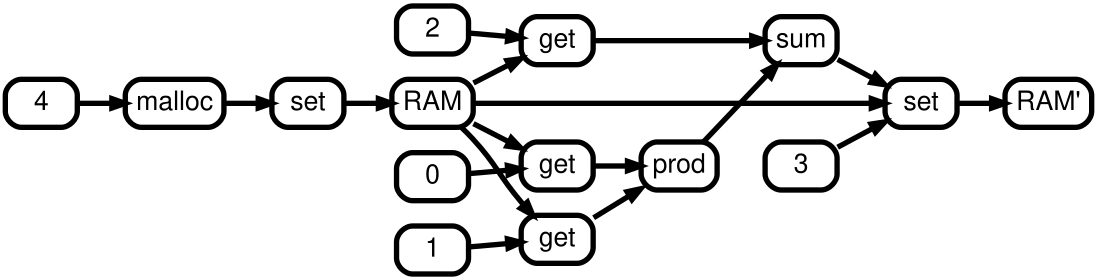
\includegraphics[scale=0.1]{rtd31}

\subsection*{2. Vector multiplication}

\begin{lstlisting}
A = malloc(4);
B = malloc(4);
C = malloc(4);
C[0] = A[0] * B[0];
C[1] = A[1] * B[1];
C[2] = A[2] * B[2];
C[3] = A[3] * B[3];
\end{lstlisting}

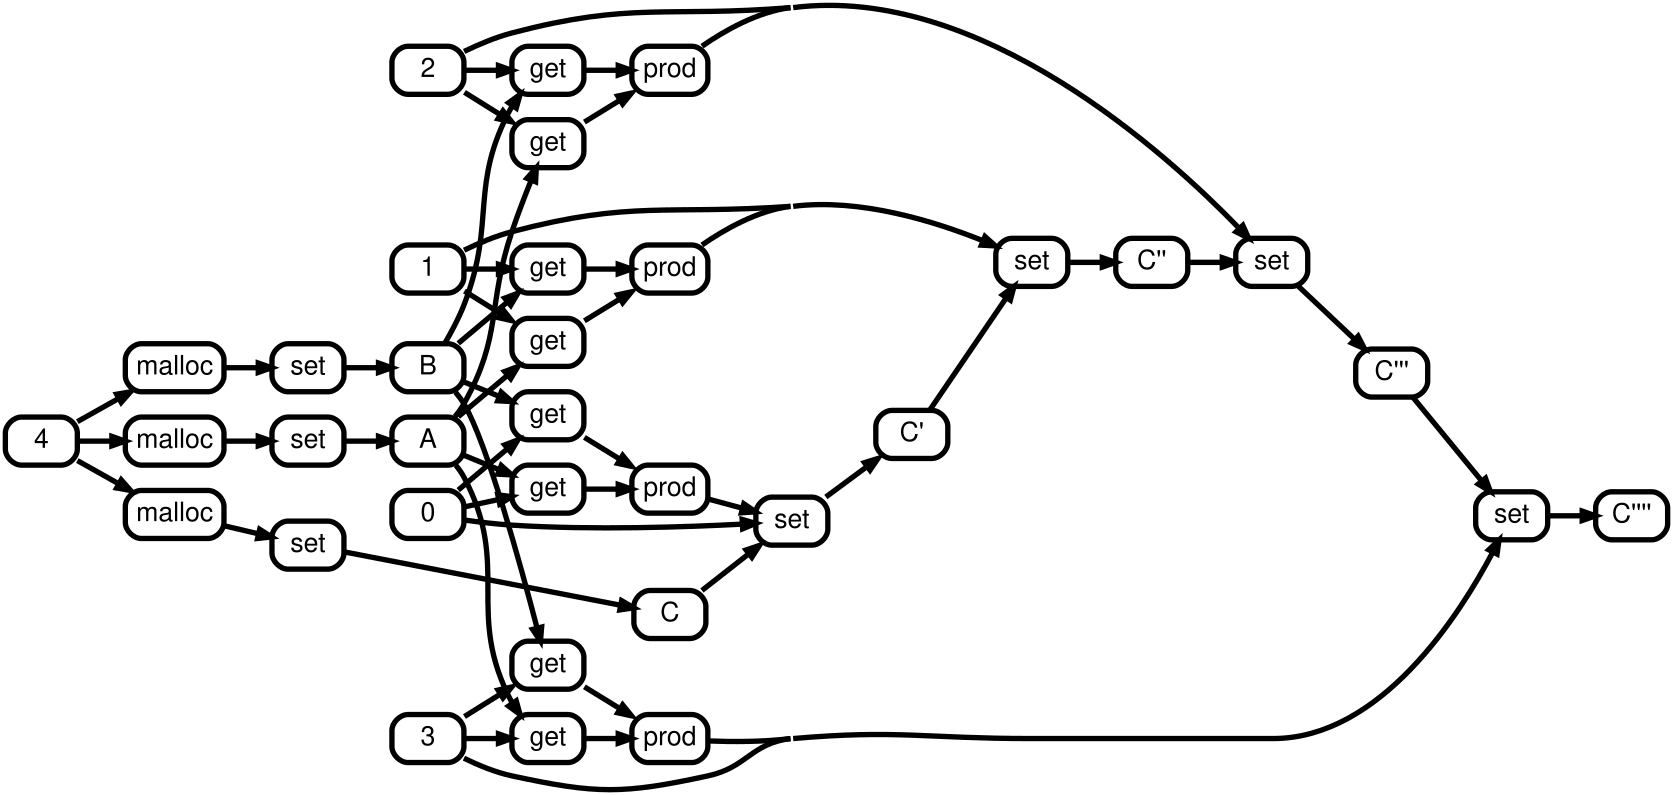
\includegraphics[scale=0.1]{rtd32}

\subsection*{3. Dot product}

\begin{lstlisting}
A = malloc(4);
B = malloc(4);
C = malloc(1);
C[0] = A[0] * B[0] +
       A[1] * B[1] +
       A[2] * B[2] +
       A[3] * B[3];
\end{lstlisting}

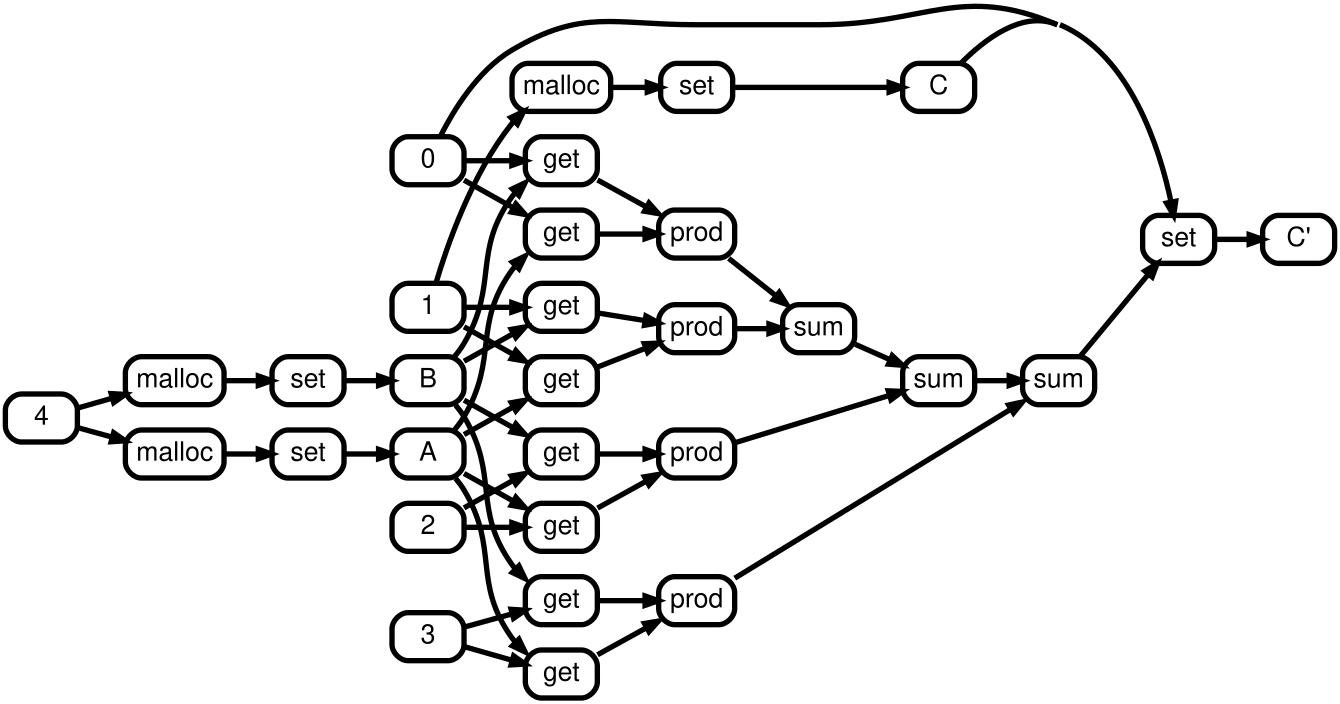
\includegraphics[scale=0.1]{rtd33}

\subsection*{4. Convolution}

\begin{lstlisting}
A = malloc(6);
W = malloc(3);
C = malloc(4);
C[0] = A[0] * W[0] + A[1] * W[1] + A[2] * W[2];
C[1] = A[1] * W[0] + A[2] * W[1] + A[3] * W[2];
C[2] = A[2] * W[0] + A[3] * W[1] + A[4] * W[2];
C[3] = A[3] * W[0] + A[4] * W[1] + A[5] * W[2];
\end{lstlisting}

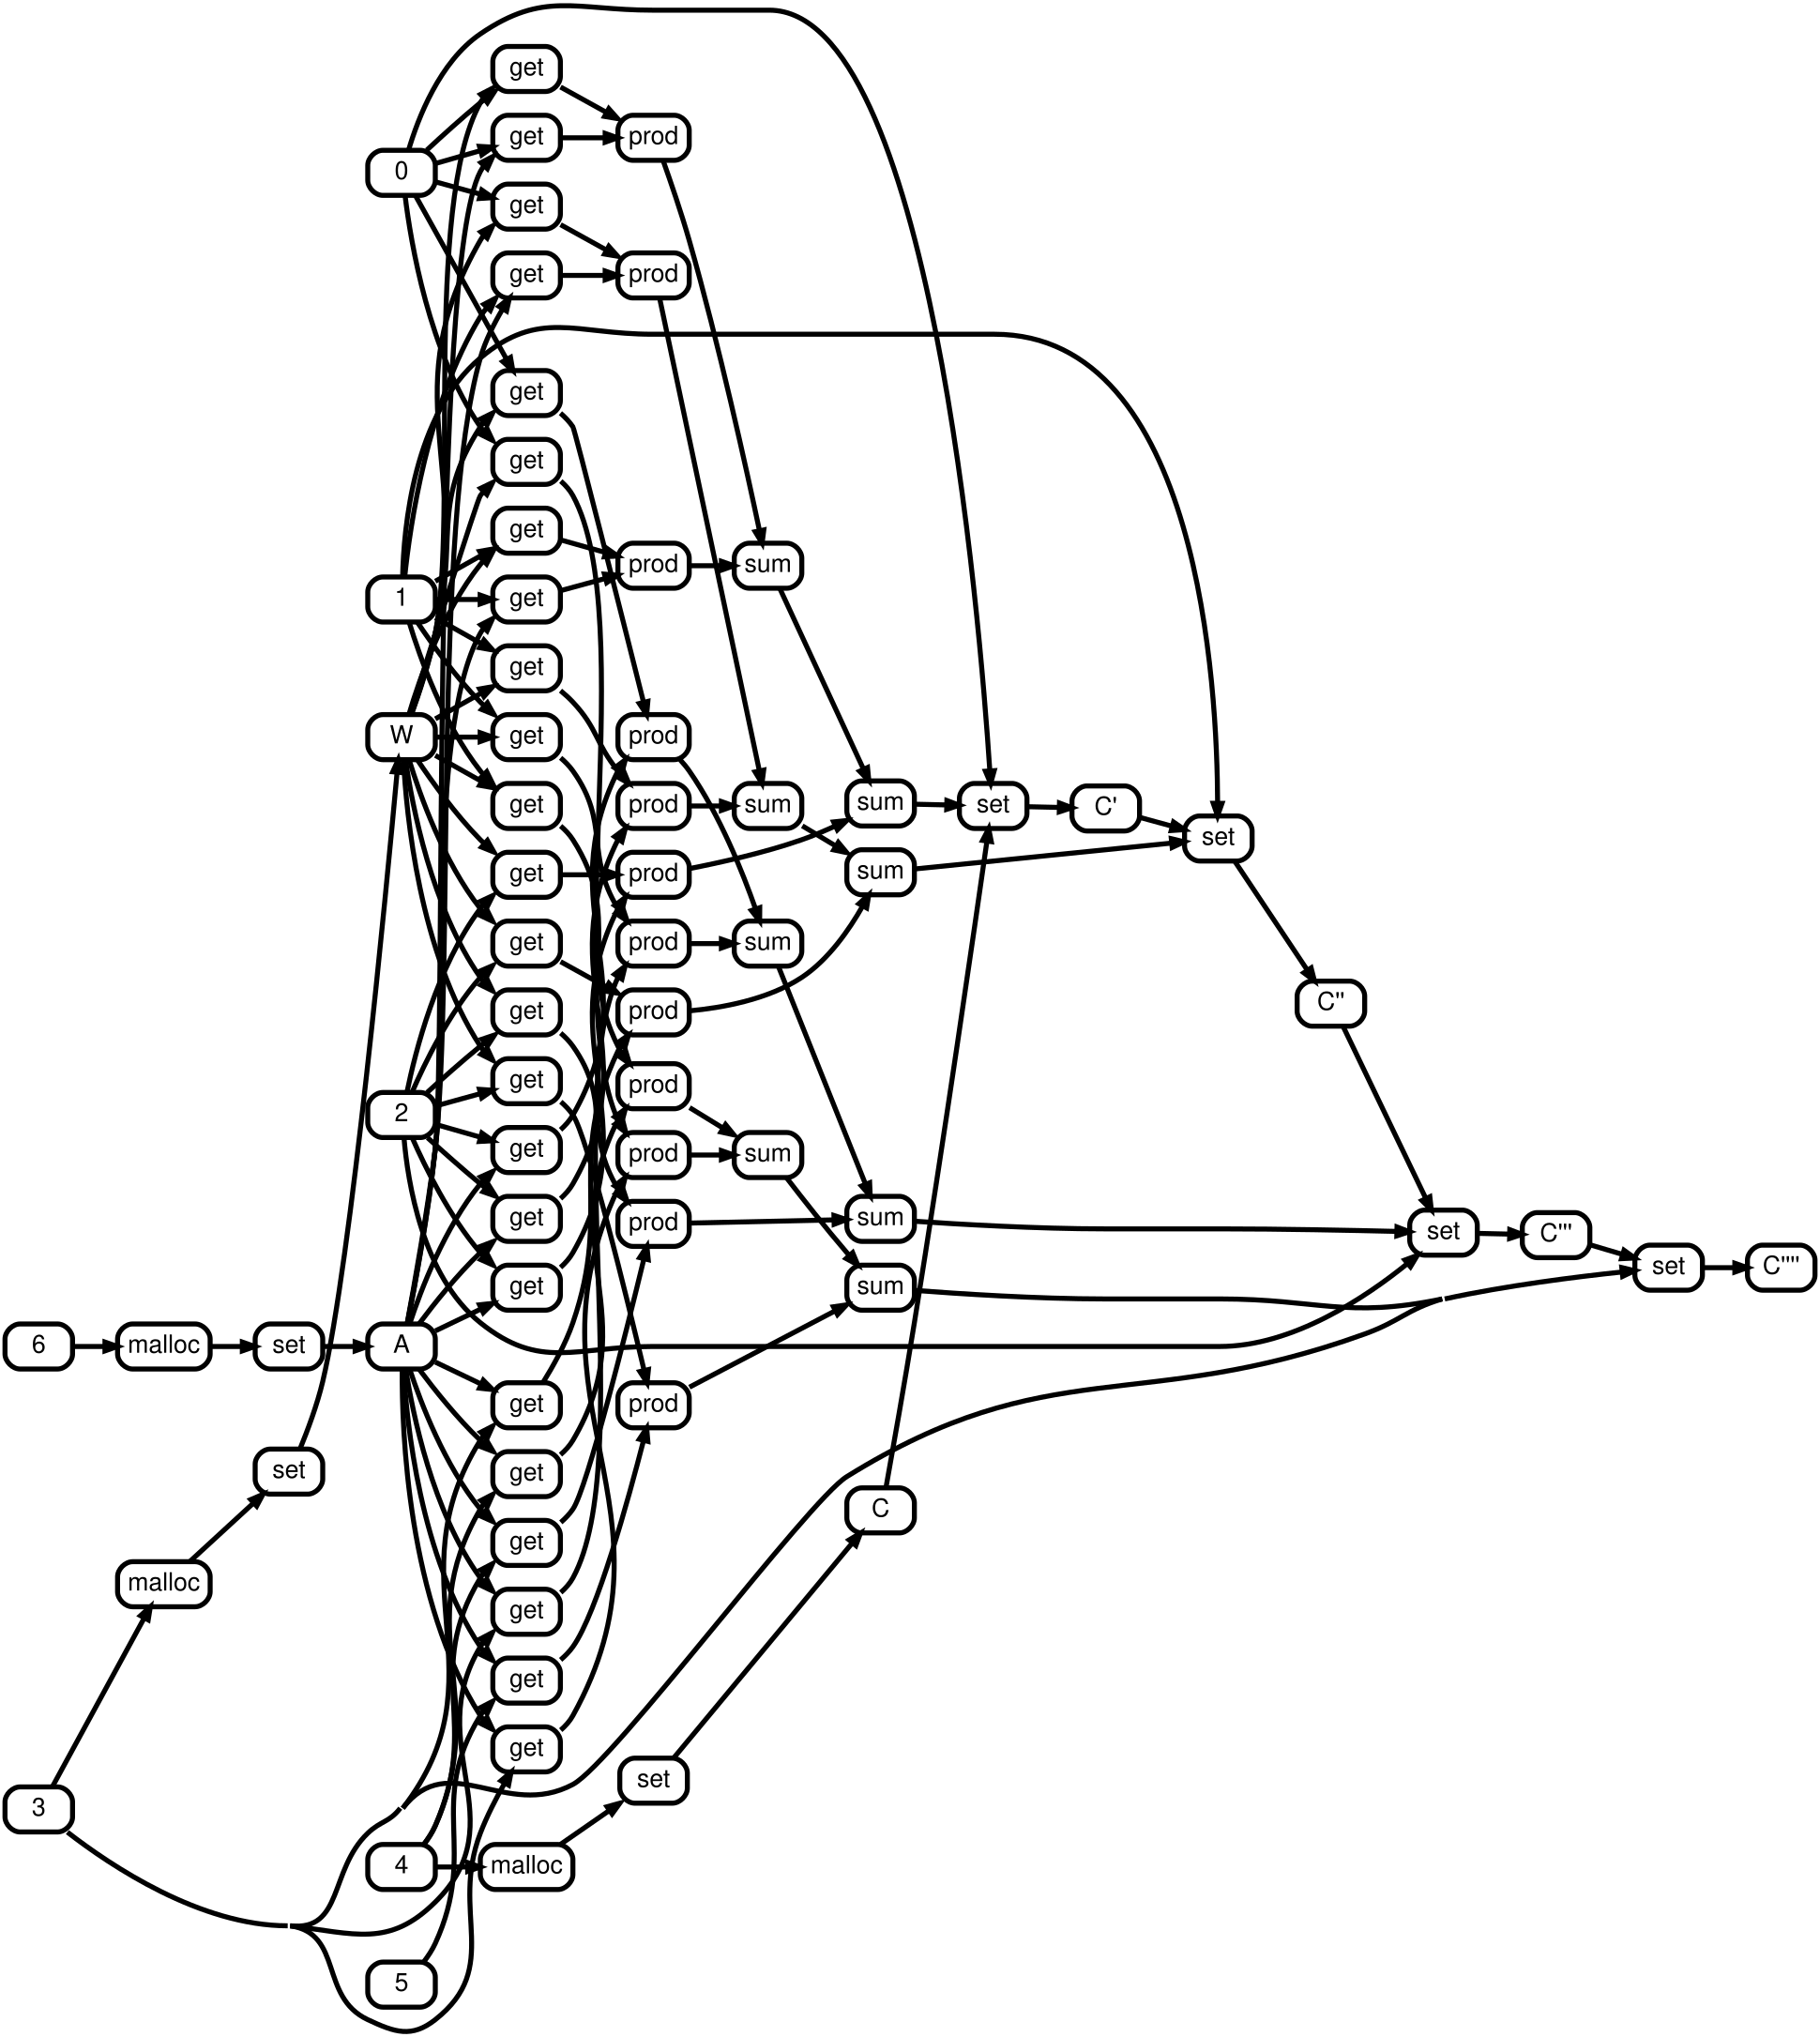
\includegraphics[scale=0.05]{rtd34}

\section*{IV. Extensions/Optimizations}

\subsection*{1. Simple variable test}

\begin{lstlisting}
I = 0;
I = 1;
I = I+J;
\end{lstlisting}

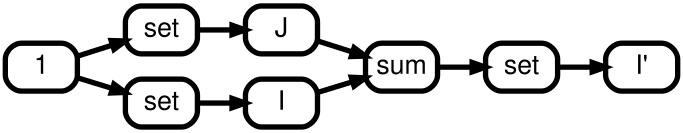
\includegraphics[scale=0.1]{rtd41}

\subsection*{2. Simple loop test}

\begin{lstlisting}
S = 0.w
for(i in 0..3) { S = S + i.w }
\end{lstlisting}

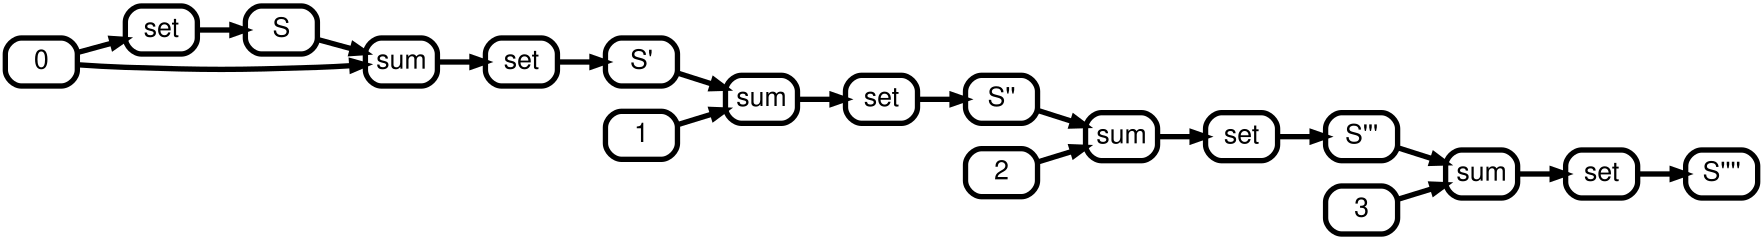
\includegraphics[scale=0.1]{rtd42}

\subsection*{3. Sum of array}

\begin{lstlisting}
A = malloc(4);
S = 0.w;
for (i in 0..3) { S += A[i] }
\end{lstlisting}

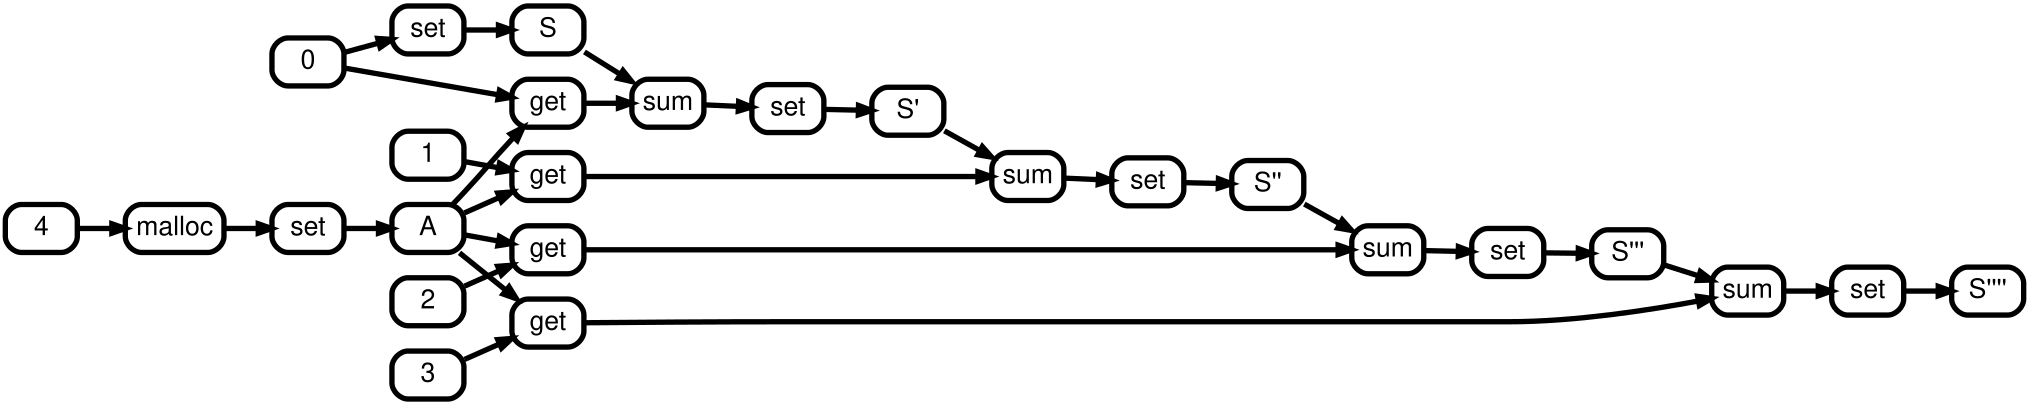
\includegraphics[scale=0.1]{rtd43}

\subsection*{4. Dot product}

\begin{lstlisting}
A = malloc(4);
B = malloc(4);
S = 0.w;
for (i in 0..3) { // 4 iterations
    S = S + A[i] * B[i];
}
\end{lstlisting}

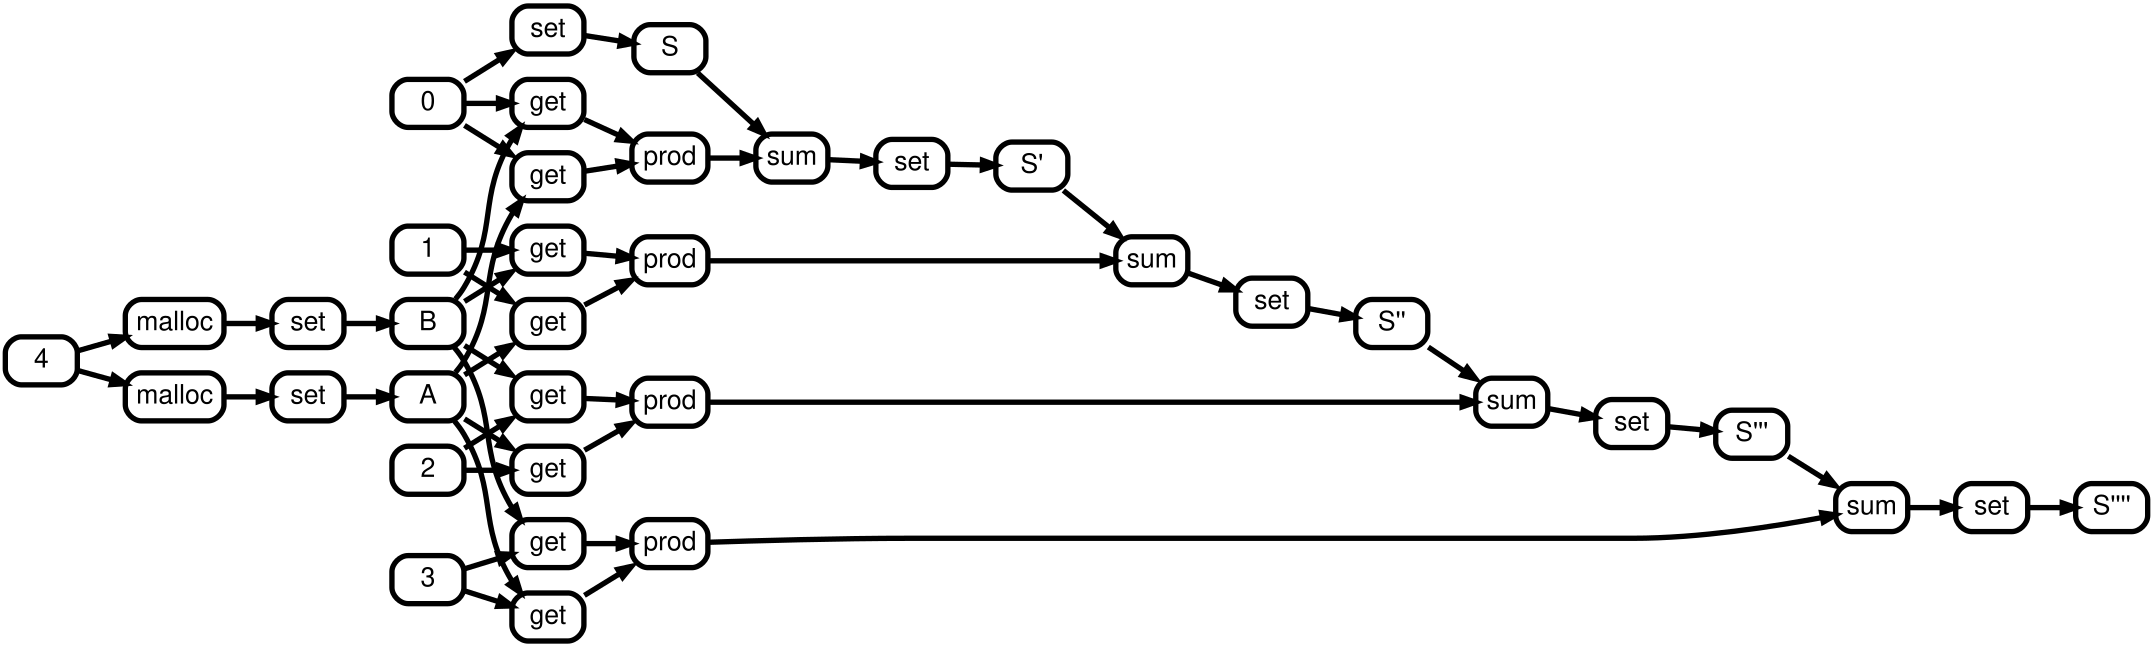
\includegraphics[scale=0.1]{rtd44}
\end{document}